\documentclass[11pt,twoside]{article}
\usepackage[left=1in,top=1in,right=1in,bottom=1in]{geometry} % Document margins
\usepackage{graphicx}
\graphicspath{ {images/} }
\usepackage{hyperref}
\usepackage{url}
\usepackage{float}

\usepackage{amssymb}
\usepackage{amsmath}
\DeclareMathOperator{\softmax}{softmax}
\DeclareMathOperator{\sigmoid}{\sigma}

\usepackage{ dsfont }
\usepackage{array}
\geometry{a4paper} % or letter or a5paper or ... etc

\title{Gradients for an RNN}
\author{Carter N Brown}
\date{%
    January 4, 2017\\%
}% delete this line to display the current date

\begin{document}
\maketitle

\section{Overview}
In this document we will go through the derivation of the gradient for an Recurrent Neural Network (RNN). The formalism and names for everything are consistent with WildML's \href{http://www.wildml.com/2015/09/recurrent-neural-networks-tutorial-part-1-introduction-to-rnns/}{RNN tutorial}. The purpose is to walk through the math in the tutorial in greater detail.

\subsection{RNN Recap}
The RNN structure can be seen below (image from WildML):

\begin{figure}[h]
\caption{RNN structure and its unfolding}
\centering
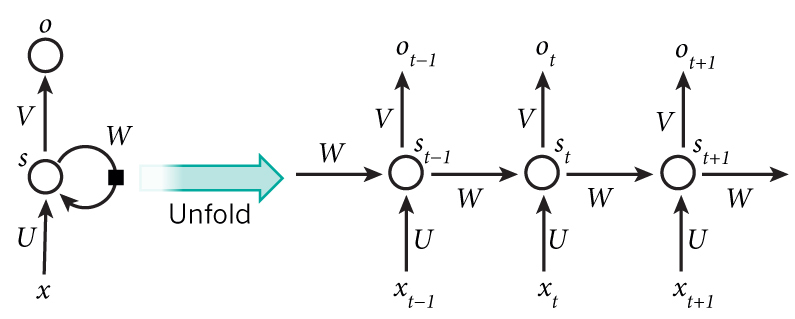
\includegraphics[width=0.75\textwidth]{rnn}
\label{rnn}
\end{figure}

\begin{subequations}
\noindent The equations for $s_t$ and $o_t$ are:
\begin{align}
s_t=\tanh(U x_t+W s_{t-1}), \\
\hat{y}_t=\softmax(V s_t).
\end{align}
\end{subequations}

\noindent Our loss function is:

\begin{equation}
\label{loss}
L(y,\hat{y})=-\frac{1}{N}\sum_{t}{}y_t\log\hat{y}_t.
\end{equation}

\noindent For the sake of computational ease later, we define:
\begin{equation}
\label{oneloss}
E_t=-y_t\log\hat{y}_t.
\end{equation}

\noindent N.B. that the loss functions are dot products between the vectors $y_t$ and element-wise logarithm of $\hat{y}_t$


\subsection{Math Recap}
The important math concepts here are \href{http://planetmath.org/einsteinsummationconvention}{Einstein Summation}, chain rule, and matrix derivatives. For the summation notation, we won't be concerned with the dual basis, i.e. all indices will be on the bottom of the variable for ease. N.B. we will not denote vectors or matrices with either arrows or boldface.

Einstein summation notation is useful here to help manage the chain rule and matrix derivatives. For example, suppose we have a function $f(x,y)$ where $x,y\in \mathbb{R}^N$. Furthermore, suppose that $x$ and $y$ are functions of $r\in\mathbb{R}$, i.e. $x=x(r)$ and $y=y(r)$. Then,

\begin{equation}
\label{chain}
\frac{\partial f}{\partial r}=\frac{\partial f}{\partial x_i}\frac{\partial x_i}{\partial r}+\frac{\partial f}{\partial y_j}\frac{\partial y_j}{\partial r}
\end{equation}

\noindent where we sum over the dummy indices $i$ and $j$. Here "dummy" means that they're only being summed over, i.e. they aren't a key part of the definition. An example of an index that isn't a dummy is $m$ in the equation $v_m=T_{m n} u_n$ (while $n$ is a dummy index).

A useful sanity checks is whether the left and right sides of the equation have the same free indices, i.e. indices that are not summed over. In our chain rule example \eqref{chain} the left side has no indices, and the right side has no free indices. In our second example, with $v_m$, both the left and right have $m$ as a free index and no others.

A nice rule of thumb for chain rule here comes with summed indices: For each pair, one index will appear in the numerator of a derivative and the other will appear in the denominator of a derivative.

Now, suppose we have a matrix $V\in\mathbb{R}^{N\times M}$ and a function $g(M)$, and we want $\frac{\partial g}{\partial V}$. Then,

\begin{equation}
\label{matcalc}
\left( \frac{\partial g}{\partial V}\right)_{i j}=\frac{\partial g}{\partial V_{i j}}.
\end{equation}

\noindent Now we can use our new summation notation to clarify definition \eqref{oneloss} for our loss function as

\begin{equation}
\label{einloss}
E_t=-y_{t_i}\log{\hat{y}_{t_i}}
\end{equation}

\section{Gradient Calculations}
The parameters of our RNN are $U, V$, and $W$, so we must compute the gradient of our loss function with respect to these matrices. This will be done in order of increasing difficulty.

\subsection{V}
The parameter $V$ is present only in the function $\hat{y}$. Let $q_t=V s_t$. Then,

\begin{equation}
\frac{\partial E_t}{\partial V_{i j}}=\frac{\partial E_t}{\partial \hat{y}_{t_k}}\frac{\partial \hat{y}_{t_k}}{\partial q_{t_l}}\frac{\partial q_{t_l}}{\partial  V_{i j}}.
\end{equation}

\noindent From our definition of $E_t$ \eqref{einloss}, we have that 
\begin{equation}
\label{e8}
\frac{\partial E_t}{\partial \hat{y}_{t_k}}=-\frac{y_{t_k}}{\hat{y}_{t_k}}.
\end{equation}

\noindent Our function $\hat{y}$ is just the sigmoid function, so

\begin{subequations}
\begin{align}
\frac{\partial \hat{y}_{t_k}}{\partial q_{t_l}}&=\left\{
	\begin{array}{lr}
	-\sigmoid(q_t)_k\sigmoid(q_t)_l, & k\neq l \\
	\sigmoid(q_t)_k\left(1-\sigmoid(q_t)_k\right), & k=l
	\end{array}
	\right. \\
\label{e9}
&=\left\{
	\begin{array}{lr}
	-\hat{y}_{t_k}\hat{y}_{t_l}, & k\neq l \\
	\hat{y}_{t_k}\left(1-\hat{y}_{t_k}\right), & k=l
	\end{array}
	\right..
\end{align}
\end{subequations}


\noindent Putting together \eqref{e8} and \eqref{e9} gives us a sum over all values of $k$ to obtain $\frac{\partial E_t}{\partial q_{t_l}}$:
\begin{subequations}
\begin{align}
-\frac{y_{t_l}}{\hat{y}_{t_l}}\left(\hat{y}_{t_l}\left(1-\hat{y}_{t_l}\right)+\sum_{k\ne l}{}\left(-\frac{y_{t_k}}{\hat{y}_{t_k}}\right)\left(-\hat{y}_{t_k}\hat{y}_{t_l}\right)  \right)
&= -y_{t_l}+y_{t_l}\hat{y}_{t_l}+\sum_{k\ne l}{}y_{t_k}\hat{y}_{t_l} \\
&= -y_{t_l} + \hat{y}_{t_l}\sum_{k}{}y_{t_k}.
\end{align}
\end{subequations}

\noindent And, if you'll recall that $y_t$ are all one-hot vectors, then that sum is just equal to 1, so
\begin{equation}
\label{diff}
\frac{\partial E_t}{\partial q_{t_l}}=\hat{y}_{t_l}-y_{t_l}
\end{equation}


\noindent Lastly, $q_t=V s_t$, so $q_{t_l}=V_{l m}s_{t_m}$. Then,
\begin{subequations}
\begin{align}
\frac{\partial q_{t_l}}{\partial V_{i j}} &= \frac{\partial }{\partial V_{i j}}\left(V_{l m} s_{t_m}\right) \\
	&= \delta_{i l}\delta_{j m}s_{t_m} \\
\label{qlV}
	&= \delta_{i l}s_{t_j}.
\end{align}
\end{subequations}

\noindent Now we combine \eqref{diff} and \eqref{qlV} to obtain:
\begin{equation}
\frac{\partial E_t}{\partial V_{i j}}=\left(\hat{y}_{t_i}-y_{t_i}\right) s_{t_j},
\end{equation}

\noindent which is recognizable as the outerproduct. Hence,
\begin{equation}
\frac{\partial E_t}{\partial V}=\left(\hat{y}_t-y_t\right) \otimes s_t,
\end{equation}
\noindent where $\otimes$ is the outer product.

\subsection{W}
The parameter $W$ appears in the argument for $s_t$, so we will have to check the gradient in both $s_t$ and $\hat{y}_t$. We must also make note that $\hat{y}_t$ depends on $W$ both directly and indirectly (through $s_{t-1}$). Let $z_t=Ux_t+Ws_{t-1}$. Then $s_t=\tanh(z_t)$.

\noindent At first it seems that by the chain rule we have:

\begin{equation}
\frac{\partial E_t}{\partial W_{ij}}=\frac{\partial E_t}{\partial \hat{y}_{t_k}}\frac{\partial \hat{y}_{t_k}}{\partial q_{t_l}}\frac{\partial q_{t_l}}{\partial s_{t_m}}\frac{\partial s_{t_m}}{\partial W_{ij}}
\end{equation}

\noindent Note that of these four terms, we have already calculated the first two, and the third is simple:
\begin{subequations}
\begin{align}
\frac{\partial q_{t_l}}{\partial s_{t_m}} &= \frac{\partial }{\partial s_{t_m}}\left(V_{lb}s_{t_b}\right) \\
&= V_{lb}\delta_{bm} \\
&= V_{lm}.
\end{align}
\end{subequations}

\noindent The final term, however, requires us to notice that there is an implicit dependence of $s_t$ on $W_{ij}$ through $s_{t-1}$ as well as a direct dependence. Hence, we have
\begin{equation}
\frac{\partial s_{t_m}}{\partial W_{ij}} \rightarrow \frac{\partial s_{t_m}}{\partial W_{ij}}+\frac{\partial s_{t_m}}{\partial s_{{t-1}_n}}\frac{\partial s_{{t-1}_n}}{\partial W_{ij}}.
\end{equation}

\noindent But we can just apply this again to yield:
\begin{equation}
\label{longchain}
\frac{\partial s_{t_m}}{\partial W_{ij}} \rightarrow \frac{\partial s_{t_m}}{\partial W_{ij}}
	+\frac{\partial s_{t_m}}{\partial s_{{t-1}_n}}\frac{\partial s_{{t-1}_n}}{\partial W_{ij}}
	+\frac{\partial s_{t_m}}{\partial s_{{t-1}_n}}\frac{\partial s_{{t-1}_n}}{\partial s_{{t-2}_p}}\frac{\partial s_{{t-2}_p}}{\partial W_{ij}}.
\end{equation}

\noindent This process continues until we reach $s_{-1}$, which was initialized to a vector of zeros. Notice that the last term in \eqref{longchain} collapses to $\frac{\partial s_{t_m}}{\partial s_{{t-2}_n}}\frac{\partial s_{{t-2}_n}}{\partial W_{ij}}$ and we can turn the first term into $\frac{\partial s_{t_m}}{\partial s_{t_n}}\frac{\partial s_{t_n}}{\partial W_{ij}}$. Then, we arrive at the compact form
\begin{equation}
\frac{\partial s_{t_m}}{\partial W_{ij}}=\frac{\partial s_{t_m}}{\partial s_{r_n}}\frac{\partial s_{r_n}}{\partial W_{ij}},
\end{equation}

\noindent where we sum over all values of $r$ less than $t$ in addition to the standard dummy index $n$. More clearly, this is written as:
\begin{equation}
\frac{\partial s_{t_m}}{\partial W_{ij}}=\sum_{r=0}^{t}\frac{\partial s_{t_m}}{\partial s_{r_n}}\frac{\partial s_{r_n}}{\partial W_{ij}},
\end{equation}

\noindent which the referenced WildML tutorial indicates as the term responsible for the vanishing gradient problem.

\noindent Combining all of these yields:
\begin{equation}
\frac{\partial E_t}{\partial W_{ij}}=\left(\hat{y}_{t_l}-y_{t_l}\right)V_{lm}\sum_{r=0}^{t}\frac{\partial s_{t_m}}{\partial s_{r_n}}\frac{\partial s_{r_n}}{\partial W_{ij}}.
\end{equation}

\subsection{U}
Taking the gradient of $U$ is similar to doing it for $W$ since they both require taking sequential derivativs of an $s_t$ vector. We have

\begin{equation}
\frac{\partial E_t}{\partial U_{ij}}=\frac{\partial E_t}{\partial \hat{y}_{t_k}}\frac{\partial \hat{y}_{t_k}}{\partial q_{t_l}}\frac{\partial q_{t_l}}{\partial s_{t_m}}\frac{\partial s_{t_m}}{\partial U_{ij}}.
\end{equation}

\noindent Note that we only need to calculate the last term now. Following the same procedure as for $W$, we find that
\begin{equation}
\frac{\partial s_{t_m}}{\partial U_{ij}}=\sum_{r=0}^{t}\frac{\partial s_{t_m}}{\partial s_{r_n}}\frac{\partial s_{r_n}}{\partial U_{ij}},
\end{equation}

\noindent and thus we have:
\begin{equation}
\frac{\partial E_t}{\partial U_{ij}}=\left(\hat{y}_{t_l}-y_{t_l}\right)V_{lm}\sum_{r=0}^{t}\frac{\partial s_{t_m}}{\partial s_{r_n}}\frac{\partial s_{r_n}}{\partial U_{ij}}.
\end{equation}

The difference between $U$ and $W$ appears in the actual implementation since the values of $\frac{\partial s_{r_n}}{\partial U_{ij}}$ and $\frac{\partial s_{r_n}}{\partial W_{ij}}$ differ.

\subsection{Total Gradient}
Since our loss function \eqref{loss} is just a summation of the $E_t$'s, we can just sum up these values we've calculated over all relevant time-steps for a given backprop to calculate our total gradient.

\end{document}